\chapter{定量脑电谱分析:基于EM算法的神经节律成分提取}

\section{引言}
神经震荡产生的兴奋和抑制塑造了大脑正常运行的传感、运动和认知过程。用新技术手段量化脑电磁记录的频谱曲线已成为研究神经震荡的主要方法之一。 一些存在的关于谱分解的文献报道了利用不具有合理统计学意义的准则来提取节律成分的手段。在本章中,我们利用Whittle似然准则和期望最大化算法分离和拟合谱曲线中的多个节律成分,我们分析发现“期望”步相当于维纳滤波(Wiener filtering)分离开多个节律成分,“最大化”步是最小化平滑惩罚和基于单调性形状约束的负Whittle似然函数,形状约束能够拟合多种不同形状的节律成分。谱曲线分解以后允许刻画各个节律的震荡幅度、共振频率、带宽、偏斜度、陡峭度和斜率。 这种方法称为$\xi\pi$模型,前后两个字母分别代表神经震荡的背景活动和多种节律峰。 我们应用这种方法到大样本的颅内脑电数据集,从某些被试被记录到的脑区推断到另一些被试未记录到的脑区,最后得到了全脑高空间分辨率频谱参数成像。这种谱参数成像可能会为神经震荡和定量电生理研究提供了常模地形图,使我们对大脑动力学有了更进一步认识。

\section{研究背景}
神经震荡形成了细胞膜电位,再由神经元群的突触后电位同步活动累积成电流,最后被记录成为头表脑电(scalp EEG)、颅内脑电(iEEG)、皮层脑电(ECoG)和脑磁(MEG)信号\citing{buzsaki2012origin}。认知过程如注意、记忆、意识和脑功能失调的出现如精神紊乱、病态心理、精神分裂,以及皮层网络的本质都可以通过对神经震荡的研究进一步解释\citing{buzsaki2004neuronal,
uhlhaas2006neural,uhlhaas2010abnormal,ward2003synchronous}。脑电磁记录的谱分析提供了大尺度神经震荡的“指纹”特征\citing{siegel2012spectral}。

当定量脑电\citing{john1977neurometrics,da1974model,zetterberg1969estimation}的概念在19世纪70年代被提出的同时,
建立能够进行频谱分解和刻画大脑节律特征的模型也成为热门研究问题。Zetterberg等利用了滤波器的概念识别频谱中的三种成分类型并用最大似然估计法估计成分的参数\citing{isaksson1981computer,wennberg1971application,
zetterberg1975analogue}。随着定量脑电中计算机辅助分析诊断\citing{john1988neurometrics}的出现,Pascual等在\cite{pascual1988parametric}提出了基于似然比检验的方法,命名为$\xi\alpha$模型,用以提取背景震荡活动$\xi$和$\alpha$节律的参数,并应用该方法到多通道谱分析。 $\xi\alpha$模型用Student-t型分布曲线\citing{walpole2011probability,
fisher1925applications,senn1994first}拟合每一个成分,频谱中只有$\alpha$峰被拟合到,该模型没有考虑其他频带的谱峰。 最近,FOOOF通过用启发式反馈拟合的方式最小化残差平方和能够拟合出1/f震荡过程的参数和不同频带多个谱峰的高斯核参数\citing{haller2018parameterizing}。

然而,我们还可从如下几点思考存在方法的不足:
1)我们还不清楚背景谱震荡是否适合描述为1/f过程\citing{abry1995wavelets}; 2)由于谱曲线上多个频带区间上谱峰形状不一,以前采用的参数化拟合例如t型曲线或者高斯核能够有效地拟合到所有的谱成分吗? 3)比着FOOOF中用的最小二乘,是否有其他更加理论合理的准则賴评估谱曲线拟合的优劣?
4)在某个认知过程中存在多少个节律(谱峰),或者说给定一个谱曲线我们要用多少谱峰来拟合?

为了回答单个谱峰形态各异的拟合问题,平滑的单模态回归由于非参数的性质和在形状上灵活的约束似乎是一个有效的方法\citing{eilers2005unimodal,pya2015shape}。 考虑到谱成分的形态各异的特性,背景震荡仅仅是一个单调下降的函数,各个谱峰可以看作先单调上升到谱峰位置再单调下降的函数。 为了找到谱估计的合理准则,Whittle似然利用单个频率下的傅里叶系数基于中心极限定理是圆周复正态分布的假设是谱成分的统计学一致的估计量\citing{whittle1953estimatio,whittle1951hypothesis}。 谱曲线拟合的关键之一是谱峰的个数,一般可以从: i)数据驱动,谱峰的个数就是出现在谱曲线中的波峰的个数, 被一个稍微的波谷隔开的相近两个波峰即视为两个谱峰,在这种情况下,最佳的拟合通过最大似然估计或者最小化残差平方和获得;ii)模型驱动,谱峰的个数不依赖于视觉上的多少,不同频带的谱峰可能是谐波,谱峰之间可能累加或者相互抵消,被稍微的波谷隔开的相近波峰可视为一个连续大谱峰,这需要从以前的神经震荡研究中获取更多的先验知识,在这种情况下最小化拟合的残差平方和可能出现过拟合或者拟合不足,这可能通过结合神经生理学先验设计出用组稀疏(group lasso\citing{yuan2006model})的期望最大化算法。

\begin{figure}[!ht]
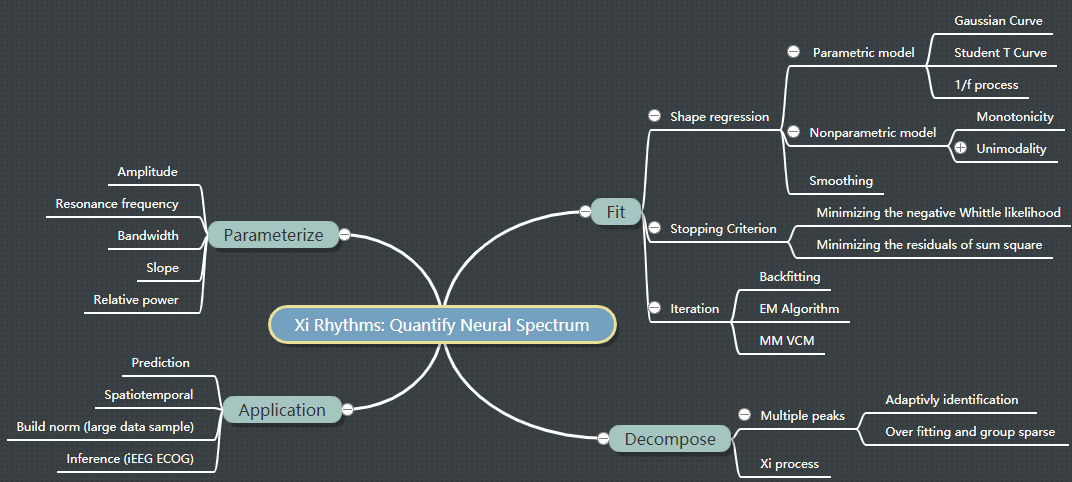
\includegraphics[width=15cm]{pic/xipi/figure1.png}
\caption{量化神经震荡谱曲线的$\xi\pi$模型综合视角}
\label{fig1}
\end{figure}

除了神经震荡谱曲线的拟合和分解,解码(量化)神经震荡谱曲线应该如\ref{fig1}中所示按照整体系统的观点进行。 拟合和分解把神经谱曲线分成几个谱成分的和,这很接近于逆问题,利用主要最小化(majorization-minimization)算法\citing{Demidenko2004,mclachlan2007algorithm,zhou2019mm,sun2016majorization}的特例期望最大化算法求解具有优势。 从谱成分中提取的参数是对神经振荡有解释意义的变量如震荡幅度、共振频率、带宽、偏斜度、陡峭度、斜率和相对于总能量的谱能量。 这使得$\xi\pi$模型应用于 1)用大型正常人群数据建立头表和源空间的震荡谱特征常模;2)作为预测认知过程和分类诊断情感紊乱的标记物;3)用iEEG或ECoG数据进行某些被试记录脑区到另一些被试未被记录到的脑区的推断\citing{owen2017towards},得到全脑高分辨率谱参数成像你呢岗位脑电磁源成像提供常模先验。

在本章中,我们发现谱曲线拟合的“期望”步骤相当于Wiener滤波器賴分析不同的谱成分,“最大化”步骤是最小化形状和平滑约束的Whittle似然函数来拟合每个谱成分。  利用公开的iEEG数据\citing{frauscher2018atlas,owen2017towards},我们得到一种全脑高分辨率谱参数成像。

\section{研究方法}
\subsection{谱曲线分解}
我们首先对脑电磁数据分段,再对每一段进行FFT变换得到傅里叶系数。 如果$y_\omega$是数据段$s(s=1,...,N_s)$在频率$\omega(\omega=1,...,N_\omega)$处的傅里叶系数,$\mathbf{z}\in{\mathbb{R}^{N_k\times{1}}}$是全为1的向量,用以进行$N_k$个$\mathbf{b}_\omega\in{\mathbb{C}^{N_k\times{1}}}$包含了在数据段s和频率$\omega$时对应于$N_k$个成分的傅里叶系数,$\Sigma_\omega=diag(\sigma_\omega)$,$\sigma_\omega=[\sigma_\omega^1,...,\sigma_\omega^{N_k}]^T$,$\epsilon_\omega\sim{N^\mathbb{C}(0,\sigma_\epsilon)}$是所有频率上具有常数方差的傅里叶系数分解残差,那么傅里叶系数分解模型是
\begin{equation}\label{eq1}
y_\omega=\mathbf{z}^T\mathbf{b}_\omega+\epsilon_\omega
\end{equation}
估计的谱是所有数据段上傅里叶系数的样本方差
\begin{equation}\label{eq2}
s_\omega=\frac{1}{N_s}\sum_{s=1}^{N_s}y_{\omega,s}^*y_{\omega,s}
\end{equation}
指定实际中计算得到的谱为$s_\omega$,理论上待拟合的谱为$\sigma_\omega$,Whittle似然\citing{pawitan1994penalized,
whittle1953estimatio,whittle1951hypothesis}定义为
\begin{equation}\label{eq3}
\ell_\omega=\sum_{\omega=1}^{N_\omega}\lbrace\log{\sigma_\omega}+\frac{s_\omega}{\sigma_\omega}\rbrace
\end{equation}

给定观测模型\eqref{eq1},脑电谱曲线分解转换为对傅里叶系数$\mathbf{b}_\omega$的估计。 利用方差成分模型和期望最大化
算法\citing{mclachlan2007algorithm},未知参数的向量为$\mathbf{\theta}_\omega^{i}=(\mathbf{\sigma}_\omega^{i};\sigma_\omega^{i})$,则完全负$\log$似然表达式为
\begin{equation}\label{eq4}
\ell_c=\sum_{\omega=1}^{N_\omega}\sum_{s=1}^{N_s}\lbrace\log{\sigma}_\epsilon^{(i)}+\mathbf{\sigma}_\epsilon^{(i)-1}\mathbf{\epsilon}_\omega^{(i)*}\mathbf{\epsilon}_\omega^{(i)}+\log\lvert\Sigma_\omega^{(i)}\rvert+\mathbf{b}_{\omega,s}^{(i)*}\Sigma_\omega^{(i)-1}\mathbf{b}_{\omega,s}^{(i)}\rbrace
\end{equation}

\subsubsection{期望步骤}
\eqref{eq1}中$y_\omega$的方差是$c_\omega^{(i)}=\Sigma_{k=1}^{N_k}\sigma_\omega^{k(i)}+\sigma_\epsilon^{(i)}$。 根据最小模最小二乘解和矩阵逆引理\citing{tarantola_inverse_2005},我们得到
\begin{equation}\label{eq5}
\mathbf{E}_{\mathbf{\theta}_\omega^{(i)}}(b_\omega^{k(i)}\mid{y}_\omega)=\sigma_\omega^{k(i)}c_\omega^{(i)-1}y_\omega
\end{equation}

显然,这里频谱中的傅里叶系数分解是一个Wiener滤波\citing{kalman1960new,Wiener1949}问题。在期望步骤,我们也可以推出
\begin{equation}\label{eq6}
d_\omega^{k(i)}=\mathbf{E}_{\mathbf{\theta}_\omega^{(i)}}(b_\omega^{k(i)}b_\omega^{k(i)*}\mid{s}_\omega)=\sigma_\omega^{k(i)}+(s_\omega-c_\omega^{(i)})c_\omega^{(i)-2}\sigma_\omega^{k(i)2}
\end{equation}
\begin{equation}\label{eq7}
e_\omega^{(i)}=\mathbf{E}_{\mathbf{\theta}_\omega^{(i)}}(\epsilon_\omega^{(i)}\epsilon_\omega^{k(i)*}\mid{s}_\omega)=\sigma_\epsilon^{(i)}+(s_\omega-c_\omega^{(i)})c_\omega^{(i)-2}\sigma_\omega^{(i)2}
\end{equation}

\subsubsection{最大化M步骤}
条件完全负$\log$似然函数是
\begin{equation}\label{eq8}
Q(\mathbf{\theta},\mathbf{\theta}^{i})=\sum_{\omega=1}^{N_\omega}\lbrace\log{\sigma_\epsilon}+\sigma_\epsilon^{-1}e_\omega^{(i)}+\sum_{k=1}^{N_k}(\log{\sigma}_\omega^k+\sigma_\omega^{k-1}d_\omega^{k(i)})\rbrace
\end{equation}
这里$\sigma_\omega^{k(i+1)}$是对$d_\omega^{k(i)}$的近似估计量,通过平滑形态约束的Whittle似然函数来拟合。

假设\eqref{eq1}中傅里叶系数分解残差的方差对所有频率上是常量,在最大化步骤可以计算为
\begin{equation}\label{eq9}
\sigma_\epsilon^{(i+1)}=\frac{1}{N_\omega}\sum_{\omega=1}^{N_\omega}e_\omega^{(i)}
\end{equation}

\subsubsection{不完全似然函数}
\begin{equation}\label{eq10}
\ell_{ic}=\sum_{\omega=1}^{N_\omega}\sum_{s=1}^{N_s}\lbrace\log{\sigma_\epsilon^{(i+1)}}+\frac{\epsilon_\omega^{(i)*}\epsilon_\omega^{(i)}}{\sigma_\omega^{(i+1)}}\rbrace
\end{equation}
直到不完全似然函数收敛,期望最大化算法完成迭代。

\subsection{谱成分拟合}
谱成分拟合指的是谱曲线分解最大化步骤对$d_\omega^{k(i)}$的拟合。如果将所有频率下对应的标量存为向量,我们得到$\mathbf{b}^{k(i)}=[d_1^{k(i)},...,d_\omega^{k(i)},...,d_{N_\omega}^{k(i)}]^T$和$\mathbf{\sigma}^{k(i+1)}=[\sigma_1^{k(i+1)},...,\sigma_\omega^{k(i+1)},...,\sigma_{N_\omega}^{k(i+1)}]^T$。\eqref{eq3}中的Whittle似然可以进一步
表示为:
\begin{equation}\label{eq11}
\ell_\omega^{(i+1)}=\mathbf{1}^T(\log{\mathbf{\sigma}}^{k(i+1)}+\mathbf{d}^{k(i)}\bigodot{\mathbf{\sigma}^{k(i+1)-1}})
\end{equation}

使用平滑形态约束\citing{eilers2005unimodal,wahba1980automatic}对$\mathbf{\sigma}^k$的估计,目标函数是
\begin{equation}\label{eq12}
\hat{\mathbf{\sigma}}^{k(i+1)}=arg\min_{\mathbf{\sigma}^{k(i+1)}}\ell_\omega^{(i+1)}+\lambda\lVert\mathbf{D}_3\mathbf{\sigma}^{k(i+1)}\rVert_2^2\qquad
s.t.\;\mathbf{\sigma}^{k(i+1)}>\mathbf{0},\mathbf{D}_1\mathbf{\sigma}^{k(i+1)}<\mathbf{0}
\end{equation}

这里$\lambda$是调整平滑程度的参数,$\mathbf{D}_3$是三阶差分矩阵平滑算子,$\mathbf{D}_1$是(修正的)一阶差分矩阵梯度算子。如果$d^{k(i)}$是单调递减曲线,$\mathbf{D}_1$就是一阶差分矩阵梯度算子,对于谱峰
成分,$\mathbf{D}_1$在谱峰最大值左侧的元素反转正负号,即谱峰最大值左右在梯度算子中分别具有负梯度和正梯度。

\subsection{参数量化}

\subsection{全脑谱参数成像}

\section{结果与讨论}
\subsection{$\xi$分解与FOOOF}
\begin{figure}[!ht]
	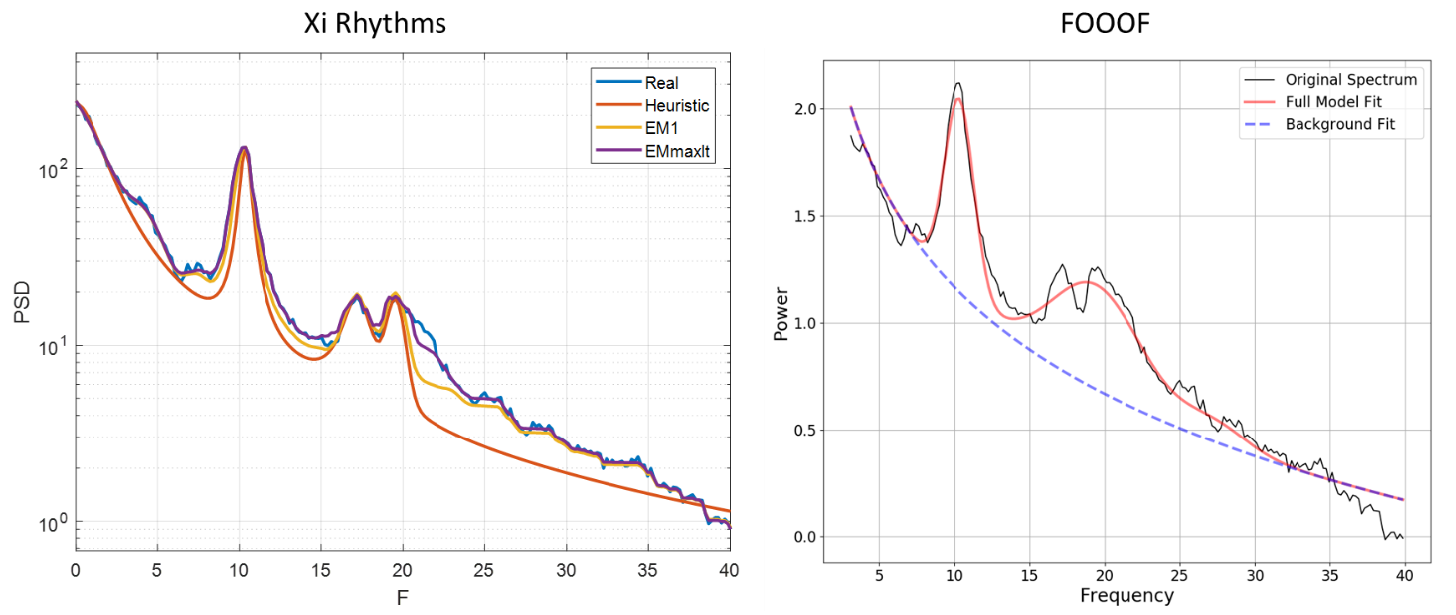
\includegraphics[width=15cm]{pic/xipi/figure3.png}
	\caption{}
	\label{fig3}
\end{figure}
\subsection{$\xi$分解的拟合}
\begin{figure}[!ht]
	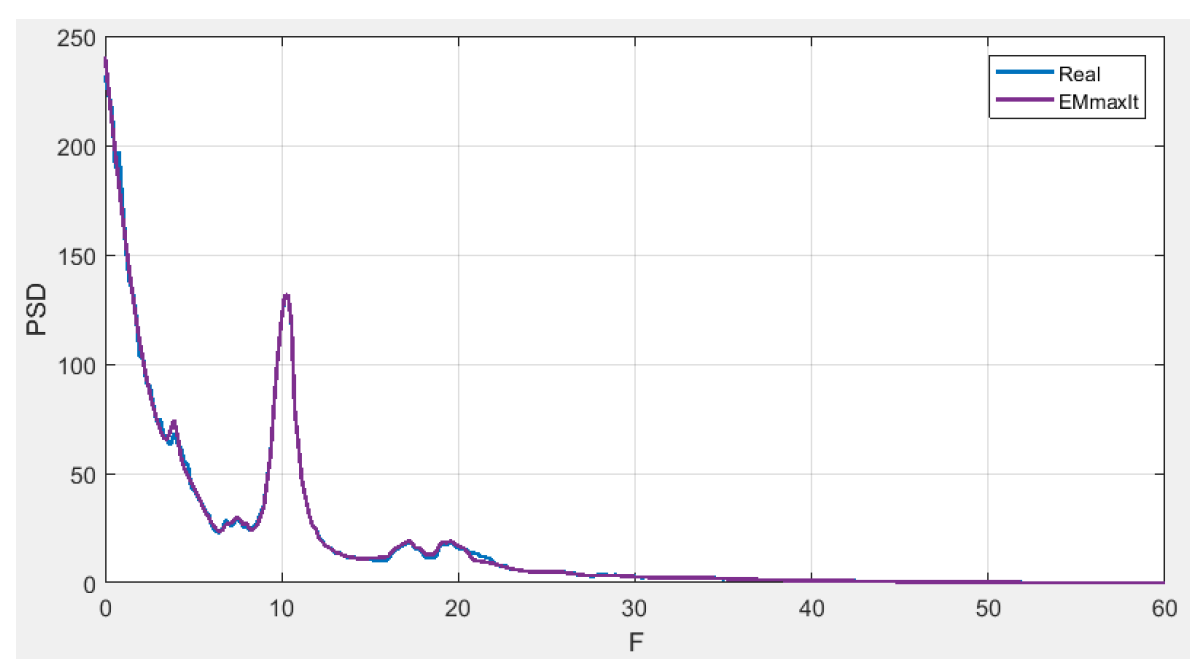
\includegraphics[width=15cm]{pic/xipi/figure3_1.png}
	\caption{}
	\label{fig3_1}
\end{figure}
\subsection{全脑高分辨率谱参数成像}
\begin{figure}[!ht]
	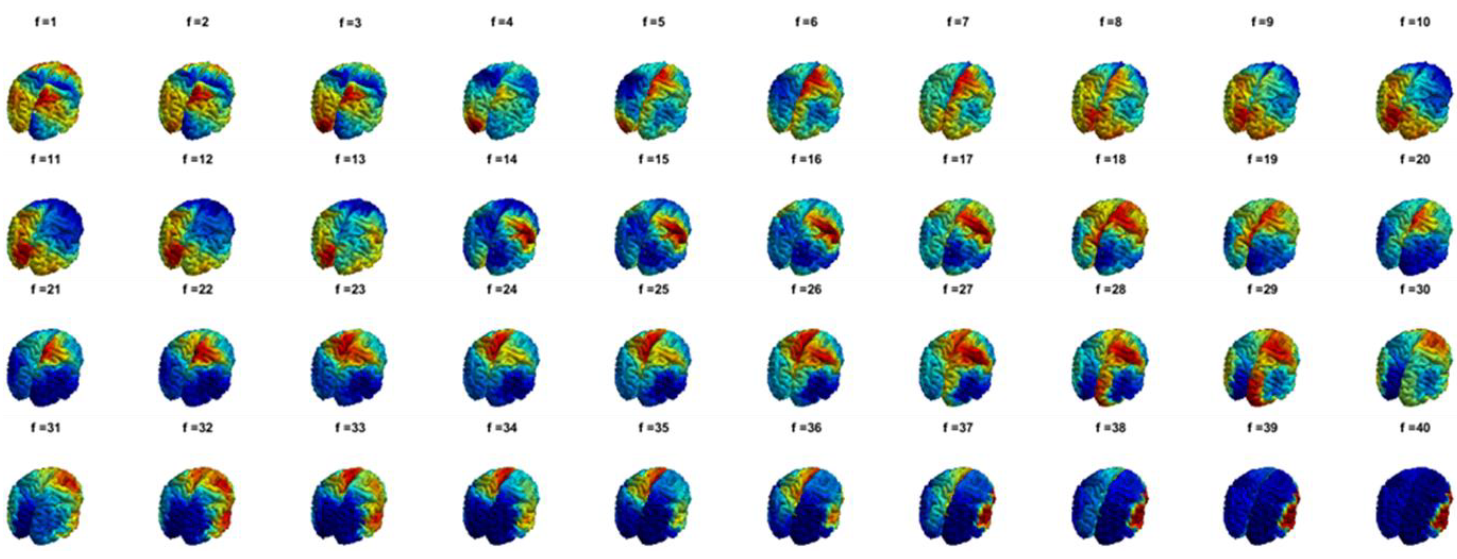
\includegraphics[width=15cm]{pic/xipi/figure4.png}
	\caption{}
	\label{fig4}
\end{figure}

\section{讨论}
There are a few problems remained to solve: (1) Add the constraint σ > 0 when using Whittle likelihood at
ordinary scale. (2) To tune the smoothing parameter, how to calculate the degree of freedom of a
nonparametric fitting? divergence of MLE (Monto Carlo)? (3) Can Whittle likelihood be transformed into a least
square, via series expansion or by log transformation (check the expansional family)? (4) Organize the Bayesian
and spectrum papers in Mendeley. (5) Review Bayesian analysis, projection estimator, Wahba smoothing and
Whittle likelihood.
The developer version of the Xi rhythms toolbox is at https://github.com/ShiangHu/SCMOPT.git.
author/funder. 

\section{本章小结}
使用期望最大化算法和基于单调性的形态回归,$\xi$节律能够把脑电功率谱分解为多个谱峰与非周期震荡谱。 在颅内脑电数据集上的应用表明$\xi$节律可能是研究神经动力学的一种有效的节律震荡分析方法。